The majority of the algorithms were implemented thinking on a distributed system approach in which data intensive processes and redundancy systems could be able to handle the provided information. The configuration employed is listed below:

\begin{itemize}
    \item Hadoop Cluster (Ubuntu System)
    \item 1 Name Node (Master)
    \item 3 Data Nodes (Slaves)
    \item Apache Spark as the processing interface with PySpark
    \item Spark Dataframes
    \item RDD’s and distributed processes
    \item Jupyter notebook for python scripting
    \item Tensorflow as the machine learning package
    \item Intended to use SparkML
    \item NLP Packages and tools:
    \item NLTK
    \item Spacy
    \item VaderSentiment
    \item Textblob
    \item Textacy
    \item Gensim
\end{itemize}

\begin{figure}[H]
   \centering
   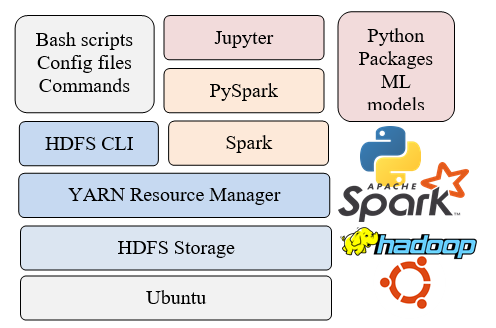
\includegraphics[width=\linewidth]{fig/serverarchitecture.png}
    \caption{Distributed system architecture}
    \label{fig:serverarchitecture}
\end{figure}

\subsection{Cryptocurrency dataset code implementation}

The code for the cryptocurrency candlestick dataset was divided in three different python files

\begin{itemize}
    \item Settings file \textbf{crypto\textunderscore params.py}
    \begin{itemize}
        \item Contains a predefined set of variables, resulted from the training and tuning of the RNN-LSTM model. The most optimistic approach ad loss function implemented can be visualized here
    \end{itemize}
    \item ML algorithm  \textbf{crypto\textunderscore utils.py}
    \begin{itemize}
        \item Contains a code snippet for the ML training model and the configuration of its layers. The way it is called and used by TensorFlow
    \end{itemize}
    \item Data set reading and training in Spark  \textbf{sprk.ipynb}
    \begin{itemize}
        \item Is a Jupyter notebook that contains the main functionality and coordination to call the settings and utils files, respectively. In addition it sets the environment to open a spark environment and connect to the Hadoop YARN resource manager, which allows the system to read the parquet files in a distributed manner.
        \item Once the files are called, the ML model is called to be trained based on the obtained data set and the result is saved in a spark json format. This allows spark to save back the trained model in the distributed system, eventually as the data keeps growing the model will be  fed in an iterative process to readjust the prediction
    \end{itemize}
\end{itemize}

\begin{figure}[H]
   \centering
   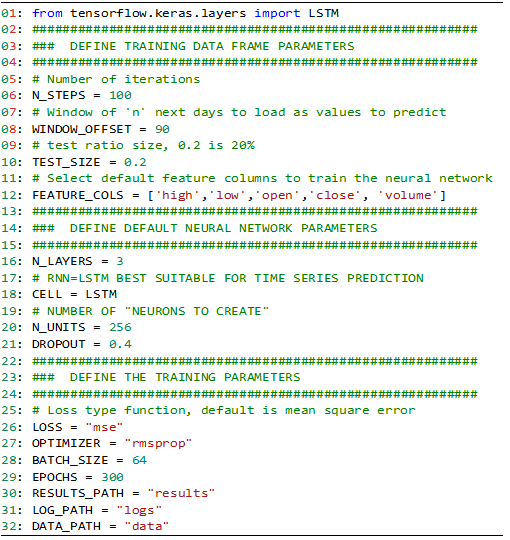
\includegraphics[width=\linewidth]{fig/CodeSnippetMLSettings.png}
    \caption{Fragment from file  crypto\textunderscore params.py}
    \label{fig:CodeSnippetMLSettings}
\end{figure}

\begin{figure}[H]
   \centering
   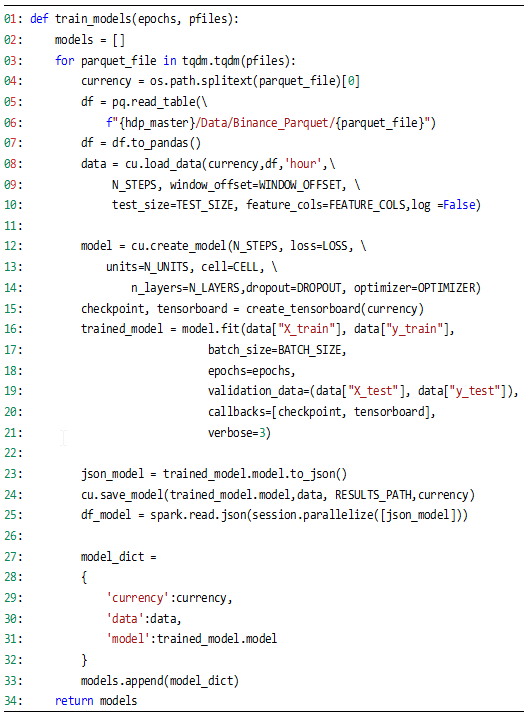
\includegraphics[width=\linewidth]{fig/CodeSnippetMLMain.png}
    \caption{Fragment from file  crypto\textunderscore utils.py}
    \label{fig:CodeSnippetMLTraining}
\end{figure}

\begin{figure}[H]
   \centering
   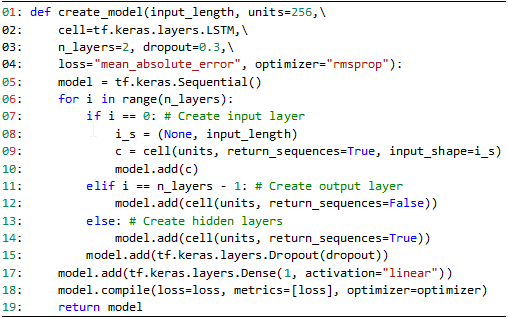
\includegraphics[width=\linewidth]{fig/CodeSnippetMLTraining.png}
    \caption{Fragment from file  crypto\textunderscore sprk.ipynb}
    \label{fig:CodeSnippetMLMain}
\end{figure}

\section{Newsfeed data set code implementation}
The newsfeed data set code required a special treatment. It consisted of two stages:

\subsubsection{Stage 1. Newsfeed data set extraction}

Since the whole data was not available on the web, a python script had to be developed in order to store such the information from the known sources. The implementation of such script is very important due to the lack of the information on the web. The script sets the basis for anyone else to use it and implement the code for any other newsfeed to assemble different data repositories. Both data set and code implementation have been published and made open for anyone to use it and improve it if required. The algorithm was developed in two scripts:
\begin{itemize}
    \item Newsfeed headings extraction
    \item Newsfeed articles extraction
\end{itemize}

\begin{figure}[H]
   \centering
   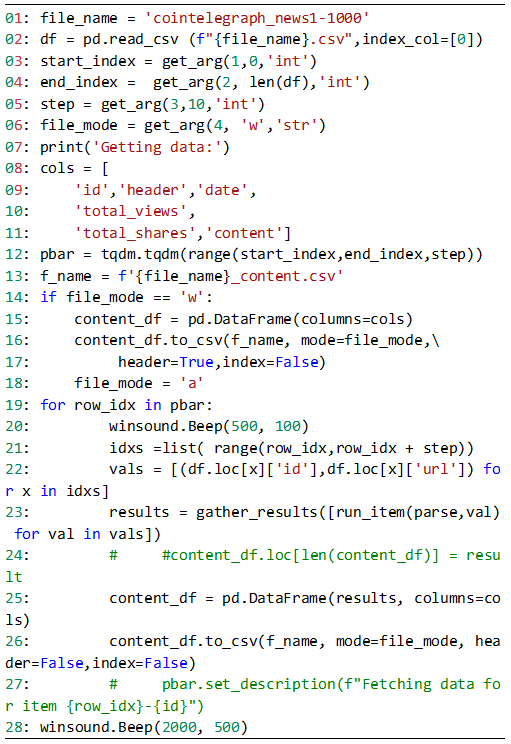
\includegraphics[width=\linewidth]{fig/CodeSnippetNewsHeadingExtraction.png}
    \caption{Code snipped for news headings extraction}
    \label{fig:CodeSnippetNewsHeading}
\end{figure}

\begin{figure}[H]
   \centering
   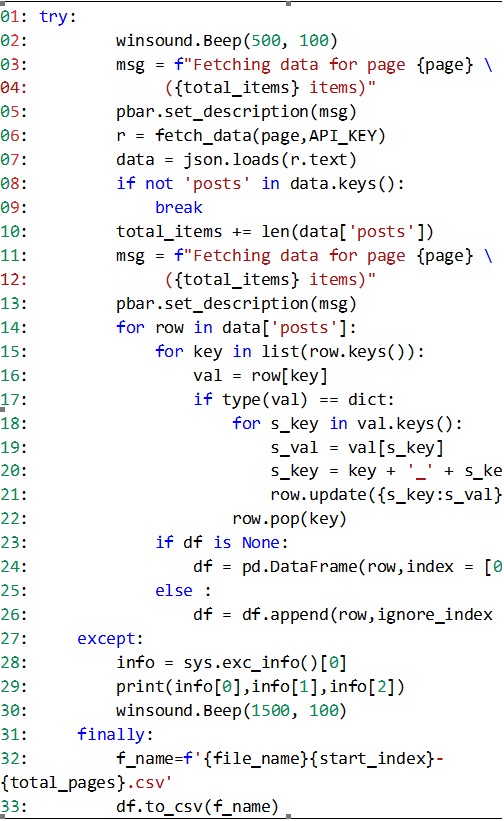
\includegraphics[width=\linewidth]{fig/CodeSnippetNewsContentExtraction.png}
    \caption{Code snipped for news articles extraction}
    \label{fig:CodeSnippetNewsContent}
\end{figure}

\subsubsection{Stage 2. Newsfeed exploration and classification}

Several attempts to classify the data set and train it to obtain relevant information that lead to decide whether an article is positive, or negative were performed. As stated in section 5.2, different approaches and analysis were tried to obtain a proper classification. Sentiment analysis, clustering, text summarization and deep learning algorithms were applied to the data set, the classification results were neutral and did not provide insightful information for the whole data set to be used and applied as an extra feature for the candlestick data set in the RNN-LTSM algorithm.

The code snippets shown below will demonstrate the use of such algorithms and the way to try to obtain useful information to tag the data set. It was observed, however, that such attempts were not enough and further text analysis was required. This is a limitation will be addressed in the next section.

\begin{figure}[H]
   \centering
   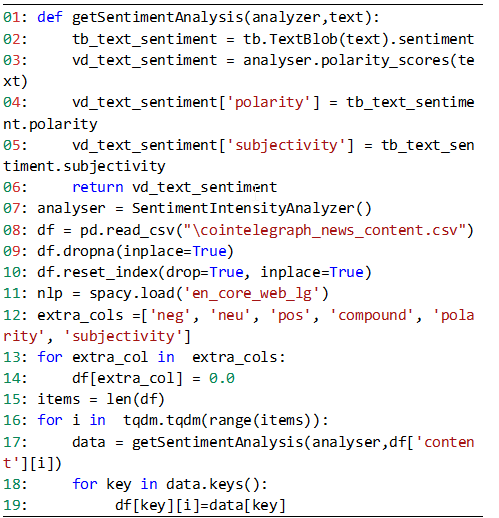
\includegraphics[width=\linewidth]{fig/CodeSnippetSentimentAnalysis.png}
    \caption{. Code snippet for sentiment analysis attempt}
    \label{fig:CodeSnippetSentimentAnalysis}
\end{figure}

\begin{figure}[t]
   \centering
   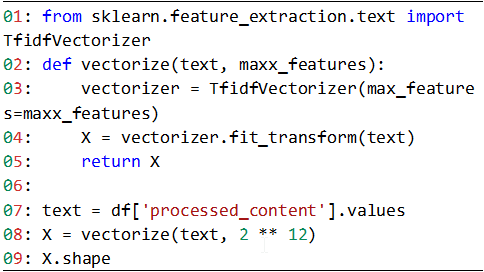
\includegraphics[width=\linewidth]{fig/CodeSnippetVectorization.png}
    \caption{Code snippet for text vectorization}
    \label{fig:CodeSnippetVectorization}
\end{figure}

\begin{figure}[H]
   \centering
   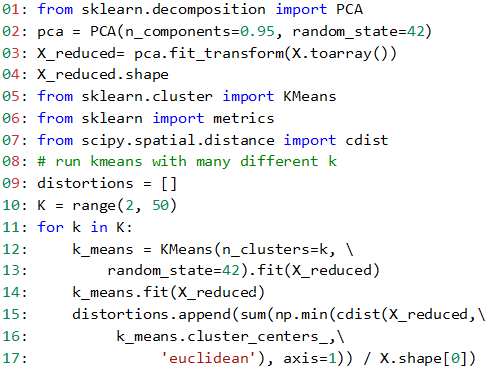
\includegraphics[width=\linewidth]{fig/CodeSnippetSentimentProcess.png}
    \caption{Code snippet for KNN clustering classification}
    \label{fig:CodeSnippetSentimentProcess}
\end{figure}


